As AWS is widely regarded as the "golden application" of the three-tier architecture, the presented component view depicts the components running on the Application Tier, or the second layer—in other words, the system's back end. The Database Tier and Presentation Tier components were segregated for better clarity. While most components are self-explanatory, some possess complex responsibilities. This section clarifies their roles within the system.

\begin{figure} [ht]
    \centering 
    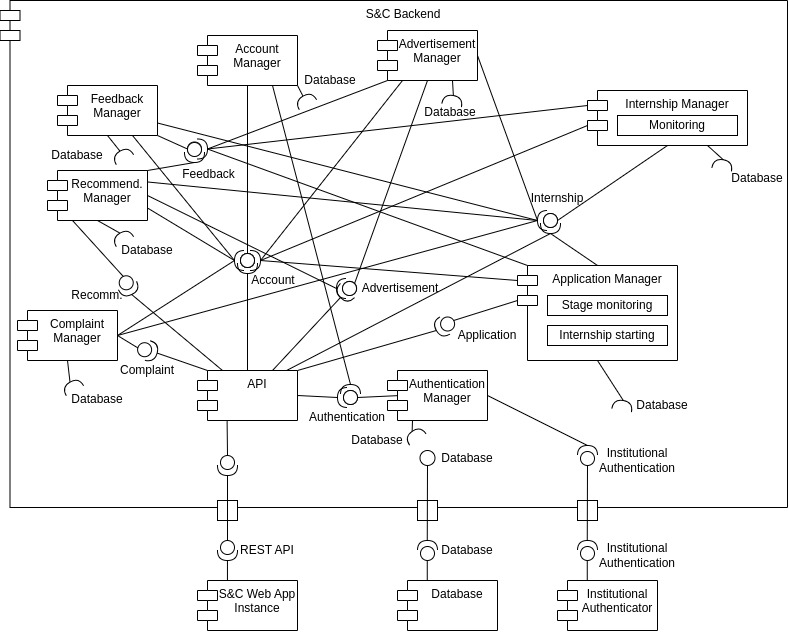
\includegraphics[width=0.9\linewidth]{DD-Latex/assets/Component Diagram/Component Diagram.jpg} 
    \caption{Component Diagram} \label{fig:Component Diagram} 
\end{figure}

\sloppy
\begin{itemize}
    \item AccountManager: Provides functionalities for managing user profiles.
    \item AdvertisementManager: Manages internship advertisements on the platform.
    \item Application Protocol Interface (API): Serves as an endpoint for receiving, routing, and transmitting data between the active Application instances and the back-end system.
    \item ApplicationManager: Processes student internship applications, including stage transitions, rejections, acceptances, and internship initialization.
    \item AuthenticationManager: Handles user authentication and routes authentication requests to institutional authenticators.
    \item ComplaintManager: Facilitates the submission of complaints during active internships.
    \item FeedbackManager: Processes feedback for users involved in internships.
    \item InternshipManager: Manages internships and the associated users. Handles user state transitions during internships and initiates feedback requests.
    \item RecommendationManager: Provides recommendations to students based on user data.
\end{itemize}

Presentation Layer and Database Layer components:
\begin{itemize} 
    \item Database: Stores platform data (Layer 3).
    \item Institutional Authenticator: An external service whose API enables institutional login for users.
    \item S\&C Web App Instance: An instance of the web application (Layer 1).
\end{itemize}

